% !TEX encoding = UTF-8 Unicode

\documentclass[a4paper, 12pt]{article}

\usepackage[T2A]{fontenc}
\usepackage[utf8x,utf8]{inputenc}
\usepackage[serbian]{babel}
\usepackage{amssymb}
\usepackage{amsmath}

\usepackage{courier}
\usepackage{listings}
\lstset{basicstyle=\footnotesize\ttfamily,breaklines=true}

\usepackage{color}
\usepackage{url}
\usepackage[unicode]{hyperref}
\hypersetup{colorlinks,citecolor=green,filecolor=green,linkcolor=blue,urlcolor=blue}
\usepackage{graphicx}
\graphicspath{ {./slike/} }
\usepackage{float}
%\usepackage{siunitx}
\usepackage{gensymb}

%-------------------------------------------------------

% Default fixed font does not support bold face
\DeclareFixedFont{\ttb}{T1}{txtt}{bx}{n}{12} % for bold
\DeclareFixedFont{\ttm}{T1}{txtt}{m}{n}{12}  % for normal

% Custom colors
\usepackage{color}
\definecolor{deepblue}{rgb}{0,0,0.5}
\definecolor{deepred}{rgb}{0.6,0,0}
\definecolor{deepgreen}{rgb}{0,0.5,0}
\definecolor{grey}{rgb}{0.5,0.1,0.1}

\usepackage{listings}

% Python style for highlighting
\newcommand\pythonstyle{\lstset{
language=Python,
basicstyle=\ttm,
otherkeywords={self},             % Add keywords here
keywordstyle=\ttb\color{deepblue},
commentstyle=\ttm\color{grey},
emph={MyClass,__init__},          % Custom highlighting
emphstyle=\ttb\color{deepred},    % Custom highlighting style
stringstyle=\color{deepgreen},
frame=t,                         % Any extra options here
showstringspaces=false            % 
}}


% Python environment
\lstnewenvironment{python}[1][]
{
\pythonstyle
\lstset{#1}
}
{}

% Python for external files
\newcommand\pythonexternal[2][]{{
\pythonstyle
\lstinputlisting[#1]{#2}}}

% Python for inline
\newcommand\pythoninline[1]{{\pythonstyle\lstinline!#1!}}
%----------------------------------------------------------

\begin{document}

\begin{titlepage}

\title{\textbf{Slobodna bacanja}}

\begin{center}
  \bfseries
  \large Matematički fakultet
  \vskip.2in
   Unvirezitet u Beogradu
  \vskip1.5in
  \emph{\huge Slobodna bacanja}
  \vskip.1in
  \small Seminarski rad iz predmeta \\Osnove matematičkog modeliranja
  \vskip.5in
  \large Matija Miličević \quad Jovana Rađenović
\end{center}

\vskip1.4in

\begin{minipage}{.3\textwidth}
  \begin{flushleft}
    \bfseries\large Profesor:\par \emph{Dr Milan Dražić}
  \end{flushleft}
\end{minipage}
\hskip.4\textwidth
\begin{minipage}{.3\textwidth}
  \begin{flushleft}
    \bfseries\large Asistent:\par \emph{Marija Ivanović}
  \end{flushleft}
\end{minipage}

\vskip1.7in

\centering
\bfseries
\Large maj 2019
\end{titlepage}

\pagebreak

\tableofcontents

\pagebreak

\section{Zadatak}

Košarkaš prilikom slobodnog bacanja izbacuje loptu sa visine koja odgovara 5/4 sopstvene visine. Ako zanemarimo trenje vazduha, i ako je ugao bacanja $\theta$, da bi lopte prošle centrom obruča potrebna je brzina izbačaja $v_\theta$. Sa istom brzinom $v_\theta$ lopta će ući u koš i za bliske uglove $[\theta_1, \theta_2]$ (a da ne dodirne obruč). Za zadatu visinu košarkaša h odrediti onaj ugao bacanja $\theta$ koji obezbeđuje maksimalnu toleranciju $\theta_2 - \theta_1$. Rezultate tabelirati za omiljeni košarkaški klub ili reprezentaciju.

\subsection{Pojmovi}

Osnovni pojmovi:

%\vskip0.2cm
%TODO

\begin{list}{}{}

\item $h$ - visina košarkaša koji izvodi slobodna bacanja;
\item $h_k$ - visina koša, $h_k = 3.05$ $m$;
\item $\theta$ - ugao izbačaja;
\item $v_\theta$ - brzina izbačaja za ugao $\theta$ pri kojoj lopta prolazi kroz centar obruča;
\item $d_c$ - rastojanje od košarkaša (y-ose) do centra obruča, $d_c = 4.19$ $m$;
%\\($4.57$ $m$ - od linije do table, $0.15$ $m$ - od table do obruča, $0.23$ $m$ - $r_l$)
\item $r_l$ - poluprečnik lopte, $r_l = \dfrac{0.75 m}{2\pi} \approx 0.1193$ $m$;
\item $r_o$ - poluprečnik obruča, $r_o = 0.23$ $m$;
\item $g$ - gravitaciona konstanta, $g = 9.81 \dfrac{m}{s^2}$;

\end{list}


\section{Modeliranje leta lopte}

Podrazumevaćemo:
\begin{itemize}

\item lopta ide dirketno ka košu, ne skreće sa putanje levo ili desno. Odnosno, nema lateralne greške pri šutu.

\item ugao $\theta$ je između $0^0$ i $90^0$:\\
\[0 < \theta < \pi/2\]

\item visina koša $h_k$ je veća od visine izbačaja košarkaša $\dfrac{_5}{^4}h$:\\
\[h_k > \dfrac{_5}{^4}h\]

\end{itemize}


Posmatraćemo centar lopte kao materijalnu tačku $L = (x,y)$ koja počinje svoj put iz tačke $(x_0,y_0) = (0,\dfrac{_5}{^4}h)$. Da bi lopta prošla kroz centar obruča u jednom trenutku mora važiti $L = C$, gde je $C = (d_c,h_k)$.\\

Pošto su visina koša i košarkaša konstantne veličine možemo da transliramo ceo sistem tako da početna tačka centra lopte bude $L = (x_0,y_0) = (0,0)$, a tačka centra obruča $C = (d_c,h_k-\dfrac{_5}{^4}h)$.
Zbog jednostavnosti zapisa uzećemo da je $H = h_k-\dfrac{_5}{^4}h$, odnosno $C = (d_c,H)$.\\

\begin{figure}[h]
\hspace*{0.9cm}
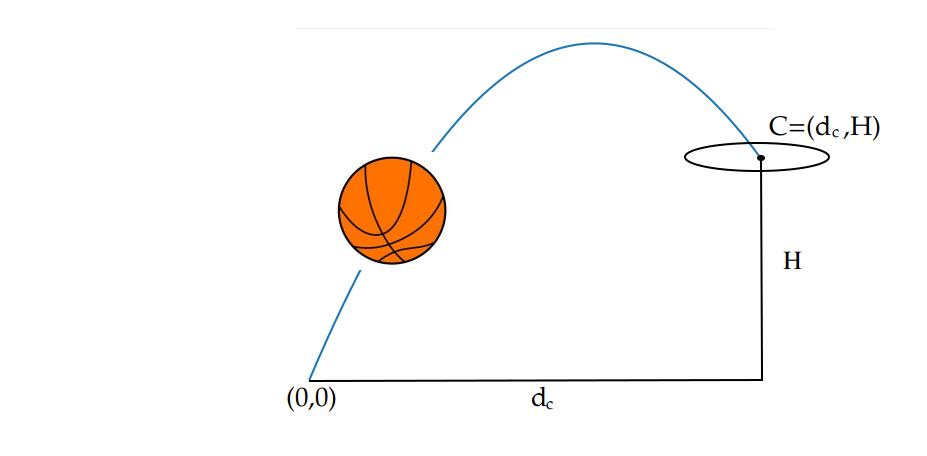
\includegraphics[width=10cm, height=5cm]{pic1}
\caption{Putanja lopte}
\end{figure}

Po ovoj slici možemo primetiti da je polazni problem u stvari jedna vrsta problema kosog hica.



\subsection{Kretanje lopte}

Nakon što je bačena, možemo primetiti da na $x$-koordinatu lopte više ne utiče nijedna sila (otpor vazduha zanemarujemo), a pošto se lopta kreće brzinom zadatom pri šutu dolazimo do zaključka da važi:\\


\[x(t) = x_0 + v_{\theta x}\cdot t\]


Gde su: $x_0 = 0$; $v_{\theta x} = v_\theta \cdot \cos \theta$; odnosno:

\begin{equation}
x(t) = v_\theta \cdot \cos \theta \cdot t
\end{equation}

Sa druge strane na $y$-koordinatu sve vreme utiče gravitacija. Uz početnu brzinu zadatu šutom možemo da zaključimo da važi:

\[y(t) = y_0 + v_{\theta y} \cdot t - \dfrac{g \cdot t^2}{2}\]

gde je $g \approx 9.81\dfrac{_m}{^{s^2}}$. Pošto važi da su: $y_0 = 0$; $v_{\theta y} = v_\theta \cdot \sin \theta$; sledi:

\begin{equation}
y(t) = v_\theta \cdot \sin \theta\cdot t - \dfrac{g}{2} \cdot t^2
\end{equation}

Dakle, koordinate centra lopte $L$ u nekom trenutku $t$ su:

\[L(t) = (x(t), y(t)) = (v_\theta \cdot \cos \theta \cdot t, v_\theta \cdot \sin \theta \cdot t - \dfrac{g}{2} \cdot t^2)\]

\subsection{Odnos brzine, daljine i ugla ($v, d, \theta$)}

Videli smo da položaj lopte zavisi od parametra vremena $t$. Nas zanima trenutak kada lopta prolazi kroz koš, odnosno $(x,y) = (d_c,H)$. Taj trenutak ćemo obeležiti sa $T$. Iz (1) i (2) sledi:

\[x(T) = v_\theta \cdot \cos \theta \cdot T = d_c\]

\[y(T) = v_{\theta} \cdot \sin \theta \cdot T - \dfrac{g}{2} \cdot T^2 = H\]

%\pagebreak

Želimo da:

\begin{enumerate}
\item Nadjemo za ugao $\theta$ takvo $v_{\theta}$ da lopta prolazi kroz centar obruča $C$
\item Nadjemo najmanji ($\theta_1$) i najveći ($\theta_2$) ugao za koji lopta bačena tom brzinom $v_{\theta}$ i dalje upada u koš
\end{enumerate}

Da bismo našli $v_{\theta}$ koristimo prethodne dve jednačine. Iz prve jednačine:

\begin{equation}
T = \dfrac{d_c}{v_\theta \cos \theta}
\end{equation}

Dakle, vidimo odnos vremena i brzine. Gledamo sad drugu jednačinu:

\[v_{\theta} \sin \theta \cdot T - \dfrac{g}{2} \cdot T^2 = H\]

\[- \dfrac{g}{2} \cdot T^2 + v_{\theta} \sin \theta \cdot T - H = 0\]

Dobili smo dakle kvadratnu jednačinu po $T$, čija su rešenja:

\[T_{1,2} = \dfrac{v_{\theta} \sin \theta \pm \sqrt[]{v_{\theta}^2 \sin^2 \theta - 2 g H}}{g}\]

Možemo da vidimo da za vrednosti ${v_{\theta}^2 \sin^2 \theta < 2 g H}$ ne postoji rešenje u skupu realnih brojeva. To znači da lopta nikada neće dostići visinu H i samim tim nećemo postići koš.
U slučaju da važi ${v_{\theta}^2 \sin^2 \theta = 2 g H}$, postoji jedno rešenje $T_1 = T_2 = T$. Ovo nam isto ne odgovara jer ne prebacujemo visinu obruča. Samo ćemo uspeti da dobacimo do centra koša odozdo. Nećemo postići pogodak.

Na kraju dolazimo do konačnog slučaja ${v_{\theta}^2 \sin^2 \theta > 2 g H}$. Dobijamo dva rešenja $T_1$ i $T_2$. Ovo znači da je lopta u letu dosegla visinu H u trenutku $T_1$, dalje stigla do najviše tačke leta i pri padu u trenutku $T_2$ prošla savršeno kroz centar obruča. Pošto nas zanima trenutak prolaska kroz obruč uzimamo veće od dva $T$.

\begin{equation}
T = \dfrac{v_{\theta} \sin \theta + \sqrt[]{v_{\theta}^2 \sin^2 \theta - 2 g H}}{g}
\end{equation}

Takođe ćemo napomenuti da ubuduće važi uslov ${v_{\theta}^2 \sin^2 \theta > 2 g H}$, tj.

\begin{equation}
{\theta} > \arcsin(\sqrt[]{\dfrac{2 g H}{v_{\theta}^2}})
\end{equation}

%\pagebreak

Nakon što izjednačimo $T$ iz (3) i (4) dobijamo:

\[\dfrac{d_c}{v_\theta \cos \theta} = \dfrac{v_{\theta} \sin \theta + \sqrt[]{v_{\theta}^2 \sin^2 \theta - 2 g H}}{g}\]

\[\dfrac{g d_c}{v_\theta \cos \theta} - v_{\theta} \sin \theta = \sqrt[]{v_{\theta}^2 \sin^2 \theta - 2 g H}\]

\[\dfrac{g^2 d_c^2}{v_\theta^2 \cos^2 \theta} - 2 g d_c \tan \theta + v_{\theta}^2 \sin^2 \theta = v_{\theta}^2 \sin^2 \theta - 2 g H\]


\[\dfrac{g^2 d_c^2}{v_\theta^2 \cos^2 \theta} - 2 g d_c \tan \theta + 2 g H = 0\]

Možemo ceo izraz da delimo sa $g$ jer znamo da je veće od 0:

\begin{equation}
\dfrac{g d_c^2}{v_\theta^2 \cos^2 \theta} - 2 d_c \tan \theta + 2 H = 0
\end{equation}

\[\dfrac{g d_c^2}{v_\theta^2 \cos^2 \theta} = 2 (d_c \tan \theta - H)\]

\[\dfrac{1}{v_\theta^2} = \dfrac{2 \cos^2 \theta (d_c \tan \theta - H)}{g d_c^2}\]

\[v_\theta^2 = \dfrac{g d_c^2}{2 \cos^2 \theta (d_c \tan \theta - H)}\]

%\vskip.4in

\begin{equation}
v_\theta = \sqrt[]{\dfrac{g d_c^2}{2 \cos^2 \theta (d_c \tan \theta - H)}}
\end{equation}

%\vskip.2in

Ovo inače predstavlja brzinu neophodnu da bi lopta pri padu prošla kroz tačku $(d_c,H)$. Naravno pri uslovu da se šutira pod uglom $\theta$.
Tokom sređivanja izraza došli smo do novog uslova $d_c \tan \theta - H > 0$, odnosno:

\begin{equation}
\theta > \arctan(\dfrac{H}{d_c})
\end{equation}

%\pagebreak

Što je geometrijski logično jer da ne važi ovaj uslov mi bi ciljali ispod koša i uvek bi prebacili daljinu obruča pre nego što bi stigli na njegovu visinu.

\begin{figure}[h]
\hspace*{1cm}
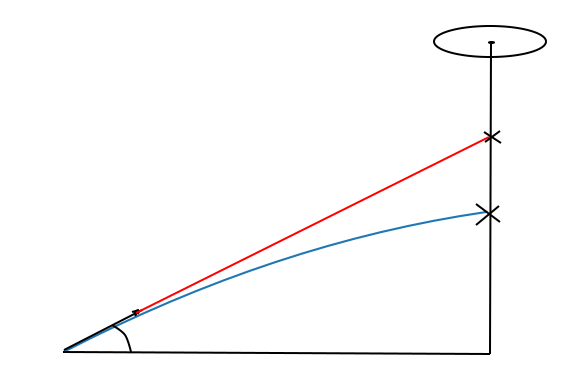
\includegraphics[width=10cm, height=5cm]{pic2}
\caption{Plava: $v=25\dfrac{m}{s^2}$; Crvena: $v=+
\infty\dfrac{m}{s^2}$}
\end{figure}

\vskip.2in

Izjednačavanjem (3) i (4) možemo da izvedemo još dve formule. Do prve dolazimo putem:

\[\dfrac{d_c}{v_\theta \cos \theta} = \dfrac{v_{\theta} \sin \theta + \sqrt[]{v_{\theta}^2 \sin^2 \theta - 2 g H}}{g}\]

\[d_c = v_\theta \cos \theta (\dfrac{v_{\theta} \sin \theta + \sqrt[]{v_{\theta}^2 \sin^2 \theta - 2 g H}}{g})\]

Odnosno:

\begin{equation}
d = \dfrac{v \cos \theta}{g}(v \sin \theta + \sqrt[]{v^2 \sin^2 \theta - 2 g H})
\end{equation}

\vskip.2in

Gde smo namerno zamenili $d_c$ i $v_\theta$ sa $d$ i $v$, jer formula važi za proizvoljne pozitivne vrednosti. Ovom formulom možemo da izračunamo daljinu koju će lopta preći pri šutu sa početnom brzinom $v$ i uglom $\theta$, pre nego što padne na visinu $H$. Jasno je da formulu (7) takođe možemo da tumačimo sa proizvoljnim $d$ umesto daljine do sredine koša. Videćemo kasnije svrhu ovih formula.

Drugu formulu dobijamo iz (6):

\[ \dfrac{g d^2}{v^2 \cos^2 \theta} - 2 d \tan \theta + 2 H = 0 \]

\[ \dfrac{g d^2 (1 + \tan^2 \theta)}{v^2} - 2 d \tan \theta + 2 H = 0 \]

\[ \dfrac{g d^2}{v^2} \tan^2 \theta - 2 d \tan \theta + 2 H + \dfrac{g d^2}{v^2} = 0 \]

\[ -g d^2 \tan^2 \theta + 2 d v^2 \tan \theta - 2 H - g d^2 = 0 \]

Ovo je očigledno kvadratna jednačina po $\tan \theta$:

\[ \tan \theta_{1,2} = \dfrac{2 d v^2 \pm \sqrt[]{4 d^2 v^4 - 4 (g d^2)(2 H + g d^2)}}{2 g d^2} \]

Nakon izvlačenja $2d$ ispred korena i skraćivanja:

\[ \tan \theta_{1,2} = \dfrac{v^2 \pm \sqrt[]{v^4 - g(2 H + g d^2)}}{g d} \]

\begin{equation}
\theta_{1,2} = \arctan (\dfrac{v^2 \pm \sqrt[]{v^4 - g(2 H + g d^2)}}{g d})
\end{equation}

Ovom formulom možemo da odredimo pod kojim uglom je potrebno izbaciti loptu da bi pri brzini $v$ prešla put $d$ pre nego što se spusti na visinu $H$.
Očigledno ako važi $v^4 - g(2 H + g d^2) < 0$ brzina lopte je premala da bi prešla daljinu $d$ pre nego što padne ispod $H$. U slučaju $v^4 - g(2 H + g d^2) = 0$ postoji jedan ugao $\theta$ kojim postižemo ovu daljinu, a za $v^4 - g(2 H + g d^2) > 0$ postoje dva ugla.


Sa formulama (7), (9) i (10) možemo da vidimo odnos brzine, daljine i ugla pri putanji naše lopte.

\pagebreak



\section{Uslovi za prolazak lopte kroz obruč}

Do sada smo loptu posmatrali kao tačku u 2-D prostoru $L = (x,y)$. Odredili smo dva uslova koja moraju biti ispunjena da bi lopta prošla kroz obruč:

\[{\theta} > \arcsin(\sqrt[]{\dfrac{2 g H}{v_{\theta}^2}}) \quad (5), \quad {\theta} > \arctan(\dfrac{H}{d_c}) \quad (8) \]

Pre nego što se pozabavimo traženjem uglova $\theta_1$ i $\theta_2$ moramo da vidimo koji još uslovi moraju biti ispunjeni da bi lopta upala u koš. Po postavci zadatka nas samo zanimaju slučajevi kada lopta ne dodiruje obruč, odbici koji ulaze u koš se ne priznaju. Pošto podrazumevamo da nema lateralne greške nas samo zanima prednji i zadnji deo obruča.

Da bi lopta prošla kroz obruč u trenutku $T$ ($y = H$) udaljenost njenog centra od prednjeg i zadnjeg dela obruča mora biti veća od poluprečnika lopte $r_l$, ali njen centar mora i dalje biti izmedju ove dve tačke. Koordinatne tačke ovih delova obruča možemo lako odrediti. Ako je centar obruča $C = (d_c,H)$, a poluprečnik obruča $r_o$, onda je bliži deo obruča $O_1 = (d_c - r_o, H)$, a dalji deo obruča $O_2 = (d_c + r_o, H)$.

Pošto je na svom putu lopta krenula da pada, možemo da primetimo da kako se njena $x$-koordinata povećava, tako se $y$-koordinata smanjuje. To znači da u trenutku $T$, kada centar lopte pada na visinu obruča, ona će imati maksimalnu $x$-koordinatu pre prolaska kroz obruč, tj. $L = (x_{max},H)$. $T$ je poslednje vreme koje razmatramo, jer nakon njega lopta je prošla kroz koš (ili nije) i nas više ne zanima njena $x$-koordinata, odnosno $t \in (0,T)$.

\begin{figure}[h]
\hspace*{1.6cm}
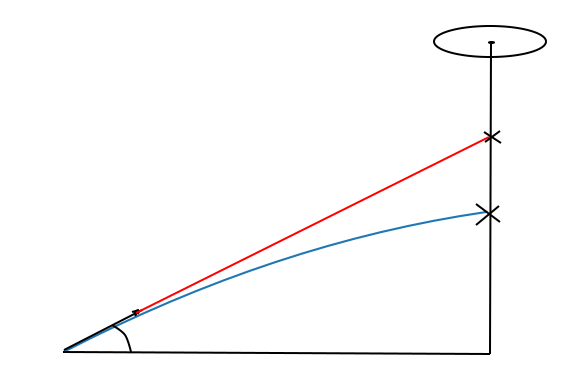
\includegraphics[scale=0.3]{pic3}
\caption{Položaj lopte u trenutku $T$}
\end{figure}

 Da bismo pronašli $x_{max}$ koristimo formulu $(9)$. Dakle, da bi lopta u trenutku $T$ prošla kroz obruč mora da važi:

\[ d_c - r_o < x_{max} - r_l \quad \land \quad x_{max} + r_l < d_c + r_o \]

\begin{equation}
d_c - r_o + r_l \quad < \quad x_{max} \quad < \quad d_c - r_l + r_o
\end{equation}


Ovo je bio uslov prolaska lopte u trenutku $T$. Nas sad zanima da li je lopta mogla udariti u obruč pre tog trenutka. Za dalji deo obruča očigledno je odgovor ne, jer ako centar lopte nije prebacio tačku $d_2$ u trenutku $T$ sigurno nije ni u nekom ranijem trenutku kada je lopta bila dalja od $O_2$. Dalje se logično postavlja pitanje za $O_1$.



\subsection{Prednji deo obruča ($O_1$)}

Udaljenost centra lopte od $O_1$ mora biti veće od poluprečnika lopte u svakom trenutku. U suprotnom to znači da je došlo do kontakta izmedju lopte i obruča. Korišćenjem pitagorine teoreme, ovo se matematički može zapisati kao:

\begin{equation}
(x - (d_c - r_o))^2 + (y - H)^2 > r_l^2
\end{equation}


\begin{figure}[h]
\hspace*{3cm}
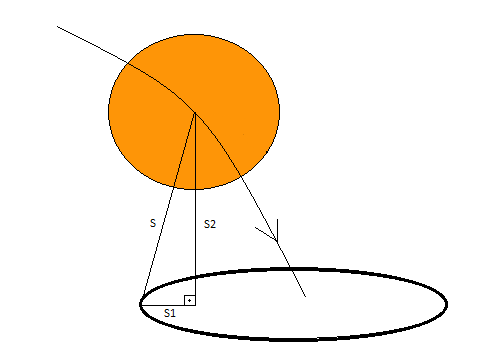
\includegraphics[scale=0.4]{pic4}
\caption{$S$: Udaljenost Lopte od $O_1$,\quad $S_1 = x - (d_c - r_o)$,\quad $S_2 = y-H$}
\end{figure}


Gde su $x$ i $y$ koordinate lopte za bilo koje $t \in (0, T)$. Ovaj uslov se geometrijski može interpretirati tako da putanja lopte ne sme da preseče kružnicu $K: (x - d_c + r_o)^2 + (y - H)^2 = r_l^2$. Menjanjem $x$ i $y$ sa $(1)$ i $(2)$ možemo da formulu kružnice pretvorimo u funkciju po $t$. Odavde ako nadjemo za $t$ bar jedno realno rešenje znamo da postoji presek putanje lopte i kružnice $K$ što znači da lopta udara u obruč i znamo za taj šut da je promašaj. Postoji samo jedan problem, dobijena formula je stepena 4:

\[ \dfrac{g^2}{4}t^4 - v \sin \theta g t^3 + (v^2 + gH)t^2 -2v((d_c-r_o) \cos \theta + H \sin \theta)t + H^2 + r_o^2 - r_l^2 - 2 d_c r_o = 0\]

\vskip.2in

Ovo se može numerički rešiti, ali postavlja se pitanje da li postoji efikasnije rešenje.
Drugi način provere uslova (12) bi bio da posmatramo loptu kao kružnicu koja se kreće pojasom širine $2r_l$.
U ovom slučaju uslov $(12)$ je isti kao i da za donju granicu ovog pojasa, dalje $DG = (x(t),y(t))$, važi da za $y = H$ sledi $x > d_c - r_o$. Putanju donje granice ovog pojasa možemo odrediti korišćenjem jediničnog vektora $\vec{n}$, normalnog na vektor brzine centra lopte $\vec{v}$. Kako je $\vec{v}(t) = \vec{L}^\prime(t)$, gde je $L(t)$ vektor položaja lopte, sledi:

\[ \vec{v}(t) = (v_0 \cos \theta, v_0 \sin \theta - gt) \]

Gde $v_0$ označava početnu brzinu šuta, koju smo ranije obeležavali sa $v$. Razlog za zamenu u ovom slučaju je da ne bismo mešali početnu brzinu $v$(tj. $v_0$) sa vektorom brzine u trenutku $t$, $\vec{v}(t)$.

\[ \vec{n}(t) = \dfrac{(- (v_0 \sin \theta - gt) ,v_0 \cos \theta)}{\| (- (v_0 \sin \theta - gt) ,v_0 \cos \theta) \|} \] 

%\pagebreak

Pošto je pravac putanje centra lopte sa leva na desno, vektor $\vec{n}$ je uperen ka nebu. Da bismo dobili putanju $DG$ treba da svakoj tački putanje lopte $L(t)$ dodamo vektor $-r_l \vec{n}$:

\[ DG(t) = L(t) - r_ln(t) = (v_0 \cos \theta t, v_0 \sin \theta t - \dfrac{g}{2} t^2)
- \dfrac{r_l (- v_0 \sin \theta + gt ,v_0 \cos \theta)}{\| (- v_0 \sin \theta + gt ,v_0 \cos \theta) \|} = \]


\[ = (v_0 \cos \theta t, v_0 \sin \theta t - \dfrac{g}{2} t^2)
- \dfrac{ (- r_l v_0 \sin \theta + r_lgt ,r_l v_0 \cos \theta)}{ \sqrt[]{v_0^2 \sin^2 \theta - 2 v_0 \sin \theta gt + g^2t^2 + v_0^2 \cos^2 \theta} } = \]


\[ = (v_0 \cos \theta t, v_0 \sin \theta t - \dfrac{g}{2} t^2)
- (\dfrac{- r_l v_0 \sin \theta + _lgt}
{\sqrt[]{v_0^2 - 2 v_0 \sin \theta gt + g^2t^2}}
,\dfrac{r_l v_0 \cos \theta}
{\sqrt[]{v_0^2 - 2 v_0 \sin \theta gt + g^2t^2}}) \implies \]

\[
DG(t) = (v_0 \cos \theta t
+ \dfrac{r_l (v_0 \sin \theta - gt)}
{\sqrt[]{v_0^2 - 2 v_0 \sin \theta gt + g^2t^2}}
, v_0 \sin \theta t - \dfrac{g}{2} t^2
- \dfrac{r_l v_0 \cos \theta}
{\sqrt[]{v_0^2 - 2 v_0 \sin \theta gt + g^2t^2}} )
\]

Mi tražimo $t$ tako da važi $DG(t) = (d_{dg}, H)$, gde je $d_{dg}$ x-koordinata donjeg dela pojasa u trenutku kada padne na visinu obruča. Ako ne postoji ili postoji samo jedno realno $t$ za koje je $y=H$ to znači da lopta ne prebacuje $O_1$, nije ispunjen uslov (12) i ne dajemo koš. Ako nadjemo dva realna rešenja za $t$ uzimamo ono veće i proveravamo da li važi $d_{dg} > d_c - r_o$. U slučaju da je ovaj uslov ispunjen tvrdimo da je lopta prebacila $O_1$ i da važi uslov (12). U suprotnom nismo postigli pogodak. Problem sa ovom metodom je taj što nije jednostavno naći $t$. Iako postoje numeričke metode za računanje $t$-a, mi nećemo koristi ovaj način.
 
\vskip.2in

Treća opcija je iterativno proveravati da li smo zakačili $O_1$, odnosno da li nije ispunjen uslov $(12)$. Znamo da za $L(t) = (x,y)$ možemo dotaći obruč samo ako važi $(d_c - r_o) - r_l < x < (d_c - r_o) + r_l $, odnosno razlika x-koordinata centra lopte $L$ i prednje ivice obruča $O_1$ je manja od poluprečnika lopte $r_l$. Nije teško odrediti $t$ za koje je $x$ u ovom rasponu. Samo koristimo formulu (3):
\[ t_1 = \dfrac{d_c - r_o - r_l}{v_\theta \cos \theta}\quad , \quad  t_2 = \dfrac{d_c - r_o + r_l}{v_\theta \cos \theta} \]

%TODO k za t u programu samo srediti.

Dalje, za mali korak $k$, $k \in  \mathbb{R}$, proveravamo za svako $t = t_1+nk$, $t \in [t_1, t_2],$ $n \in  \mathbb{N} \cup \{0\}$, da li važi uslov $(12)$. Ovde je $n+1$ broj provera koje želimo da izvršimo. Sledi da ako želimo da izvršimo $n$ provera važiće $t_2 = t_1 + (n-1)k$, odnosno $k = \dfrac{t_2 - t_1}{n-1}$. U radu smo se odlučili za 11 provera, tako da nam je $k = \dfrac{t_2 - t_1}{10}$
U slučaju da postoji $t$ za koje ne važi $(12)$ proglašavamo da je šut promašaj, inače pogodak.
Dakle, uslovi koji moraju biti ispunjeni da bismo postigli pogodak su (5), (8), (11) i (12).

%\[{\theta} > \arcsin(\sqrt[]{\dfrac{2 g H}{v_{\theta}^2}}) \quad (5) \quad \quad \textbf{;} \quad \quad {\theta} > \arctan(\dfrac{H}{d_c})  \quad (8)\]

%\[ \quad \quad d_1 < x_{max} < d_2 \quad (11) \quad \quad \textbf{;} \quad \quad (x - d_c + r_o)^2 + (y - H)^2 > r_l^2  \quad (12) \]




\section{Uglovi $\theta_1$ i $\theta_2$}

Pretpostavimo da $\theta \in (0,\pi/2)$ ispunjava uslove za pogodak. Postavlja se pitanje kako da odredimo $\theta_1$ i $\theta_2$ za dati ugao $\theta$?

Očigledan način je da iskoristimo formulu (10). Na taj način dobijamo dva kandidata:

\[ \overline\theta_1 = \arctan (\dfrac{v_\theta^2 \pm \sqrt[]{v_\theta^4 - g(2 H + g (d_c - r_o + r_l)^2)}}{g (d_c - r_o + r_l)}) \]

\[ \overline\theta_2 = \arctan (\dfrac{v_\theta^2 \pm \sqrt[]{v_\theta^4 - g(2 H + g (d_c + r_o - r_l)^2)}}{g (d_c + r_o - r_l)}) \]

U slučaju da dobijemo dva ugla za $\overline\theta_1$ ili $\overline\theta_2$ uzimamo onaj koji je bliži $\theta$.
Problem sa ovom metodom je što uzimamo u obzir samo uslov prolaza (11), ne vršimo proveru da li važe ostali uslovi (5), (8) i (12). Umesto da ih posmatramo kao rešenja, $\overline\theta_1$ i $\overline\theta_2$ će nam predstavljati granicu. Znamo za $\theta_1$ i $\theta_2$ da se nalaze u rasponu $\theta_1 \in (\overline\theta_1, \theta)$ i $\theta_2 \in (\theta, \overline\theta_2)$. Dalje možemo grubom silom da idemo od $\overline\theta_1$ i $\overline\theta_2$ ka $\theta$, pomerajući se za ugao $k$, i prvi ugao koji ispunjava sve uslove proglašavamo za $\theta_1$, odnosno $\theta_2$.

%\vskip.1in
%umesto od $\overline\theta_1$, $\overline\theta_2$

%TODO Većinom sređeno.

Jednostavnije je da počnemo od $\theta$. Za korak $k$ udaljavamo se od $\theta$ u oba smera. Čim naiđemo na ugao koji ne zadovoljava uslove, uzimamo prvi prethodni koji je zadovoljavao. Tako u oba smera, i te uglove proglašavamo za $\theta_1$ i $\theta_2$. Zbog brzine programa, radićemo dve provere. Prvo ćemo uzeti $k = 1\degree$ i ići od $\theta$ do prvog $\theta_1$ (ili $\theta_2$), zovimo ga $\theta_1'$. Potom ćemo uraditi proveru za $k = 0.01\degree$ od $\theta_1'$ do $\theta_1$ koje ćemo prihvatiti za naše $\theta_1$. Tako je rađeno u ovom radu. Za $\theta_2$ postupak je analogan.



\section{Traženje optimalnog $\theta$}

%TODO

Jednostavan i očigledan model rešenja je da za svaki mogući ugao $\theta$ nadjemo $\theta_1$ i $\theta_2$ i da kao optimalni ugao izaberemo onaj čija je razlika $\theta_2 - \theta_1$ maksimalna. Zbog toga što uglova $\theta \in (0,\pi/2)$ postoji beskonačno, koristićemo korak $k$ i tražićemo $\theta$ u obliku $ \theta = \theta_{min} + nk,$ $\theta \in (\theta_{min},$ $\theta_{max}),$ $n \in  \mathbb{N}$. Ugao $\theta_{min}$ predstavlja minimalno $\theta$ za koje možemo pogoditi koš u odnosu na pravilo (8), odnosno $\theta_{min} = \arctan(\dfrac{H}{d_c}) + 1 \degree$, gde smo dodali $1$ stepen da ne bi doslo do deljenja nulom pri računu u formuli (7). U radu smo odlučili da za $\theta_{min}$ uzmemo maksimum između prethodne formule i $20\degree$, $\theta_{min} = \max(\arctan(\dfrac{H}{d_c}) + 1 \degree,$ $20\degree)$. Ovo je odlučeno zato što u rasponu visine košarkaša od $0$ do $3$ metra svi optimalni uglovi su veći od $20\degree$. Za $\theta_{max}$ očigledan kandidat je $\pi/2$, ali kao i za $\theta_{min}$ ograničićemo sa na $70 \degree$ iz razloga što su optimalni uglovi manji za košarkaše do 3 metra.

Veoma je bitno da odredimo dovoljno mali korak $k$, u suprotnom nećemo postići precizne rezultate. U radu smo se odlučili za $k = 0.01$, tako da imamo preciznost do na drugu decimalu. Moguća varijanta ovog modela je da nakon što nadjemo $\theta$, smanjimo $k$ i gledamo okolinu $(\theta - k_{staro},$ $\theta + k_{staro})$ za novo optimalno $\theta$. Ovo nismo radili.

Vremenska složenost ovog rešenja je na taj način $O(n \cdot m \cdot l)$ gde je $n$ broj uglova $\theta$, $m$ prosek broja uglova $\theta_1$ i $\theta_2$, a $l$ broj vremenskih trenutaka ($t$-ova) za koje proveravamo uslov $(12)$. U zavisnosti od veličine koraka koji izaberemo imaćemo kompromis između preciznosti i dužine rada programa.

\pagebreak



\section{Programski kod (Python)}

%\begin{enumerate}

\large \textbf{1) Program koji traži uglove $\theta_1$ i $\theta_2$ za dato $\theta$:}
\pythonexternal[language=Python]{teta1_2.py}

%\pagebreak
\vskip.5in

\large \textbf{2) Program koji traži optimalni ugao $\theta$ (poziva 1):}
\pythonexternal[language=Python]{optimalni_ugao.py}

%\end{enumerate}

%\pagebreak



\section{Tabela: Dallas Mavericks}

\begin{table}[h]
\begin{center}
 \begin{tabular}{|p{0.7cm}|p{5cm}|p{2cm}|p{2cm}||} 
 \hline
 \# & Prezime, Ime & Visina & Ugao\\ [0.7ex]
 \hline
 37 & Antetokounmpo, Kostas & \quad 2.08 m & \quad 53.86\degree \\  %53.8604
 \hline 
 
 5 & Barea, J. J. & \quad 1.83 m & \quad 55.48\degree \\ %55.4775
 \hline
 
 45 & Broekhoff, Ryan & \quad 2.01 m & \quad 54.28\degree \\ %54.2785
 \hline
 
 13 & Brunson, Jalen & \quad 1.91 m & \quad 54.98\degree \\ %54.9850
 \hline
 
 23 & Burke, Trey & \quad 1.85 m & \quad 55.37\degree \\ %55.3697
 \hline
 
 77 & Dončić, Luka & \quad 2.01 m & \quad 54.28\degree \\ %54.2785
 \hline
 
 10 & Finney-Smith, Dorian & \quad 2.03 m & \quad 54.19\degree \\ %54.1940
 \hline
 
 11 & Hardaway, Tim & \quad 1.98 m & \quad 54.52\degree \\ %54.5246
 \hline
 
 34 & Harris, Devin & \quad 1.91 m & \quad 54.98\degree \\ %54.9850
 \hline
 
 44 & Jackson, Justin & \quad 2.03 m & \quad 54.19\degree \\ %54.1940
 \hline
 
 42 & Kleber, Maxi & \quad 2.11 m & \quad 53.65\degree \\ %53.6452
 \hline
 
 1 & Lee, Courtney & \quad 1.96 m & \quad 54.65\degree \\ %54.6478
 \hline
 
 3 & Macon, Daryl & \quad 1.91 m & \quad 54.98\degree \\ %54.9850
 \hline
 
 50 & Mejri, Salah & \quad 2.18 m & \quad 53.22\degree \\ %53.2200
 \hline
 
 6 & Porziņģis, Kristaps  & \quad 2.21 m & \quad 53\degree \\ %53.0021
 \hline
 
 7 & Powell, Dwight & \quad 2.11 m & \quad 53.65\degree \\ [1ex] %53.6452 
 \hline

\end{tabular}
\label{tabela 1}
\caption{Optimalno $\theta$ za roster Dallas Mavericks-a}
\end{center}
\end{table}

\end{document}